\documentclass{article}

\usepackage{graphicx}
\usepackage{tikz}
\usepackage{tikzsymbols}
\usetikzlibrary{calc,patterns,shapes.geometric}
\pagestyle{empty}
\usepackage[margin=0pt]{geometry}
\geometry{papersize={14in,12in}}

\def\centerarc[#1](#2)(#3:#4:#5){\draw[#1] ($(#2)+({#5*cos(#3)},{#5*sin(#3)})$) arc (#3:#4:#5);}

\begin{document}
	\begin{figure}
		\centering
		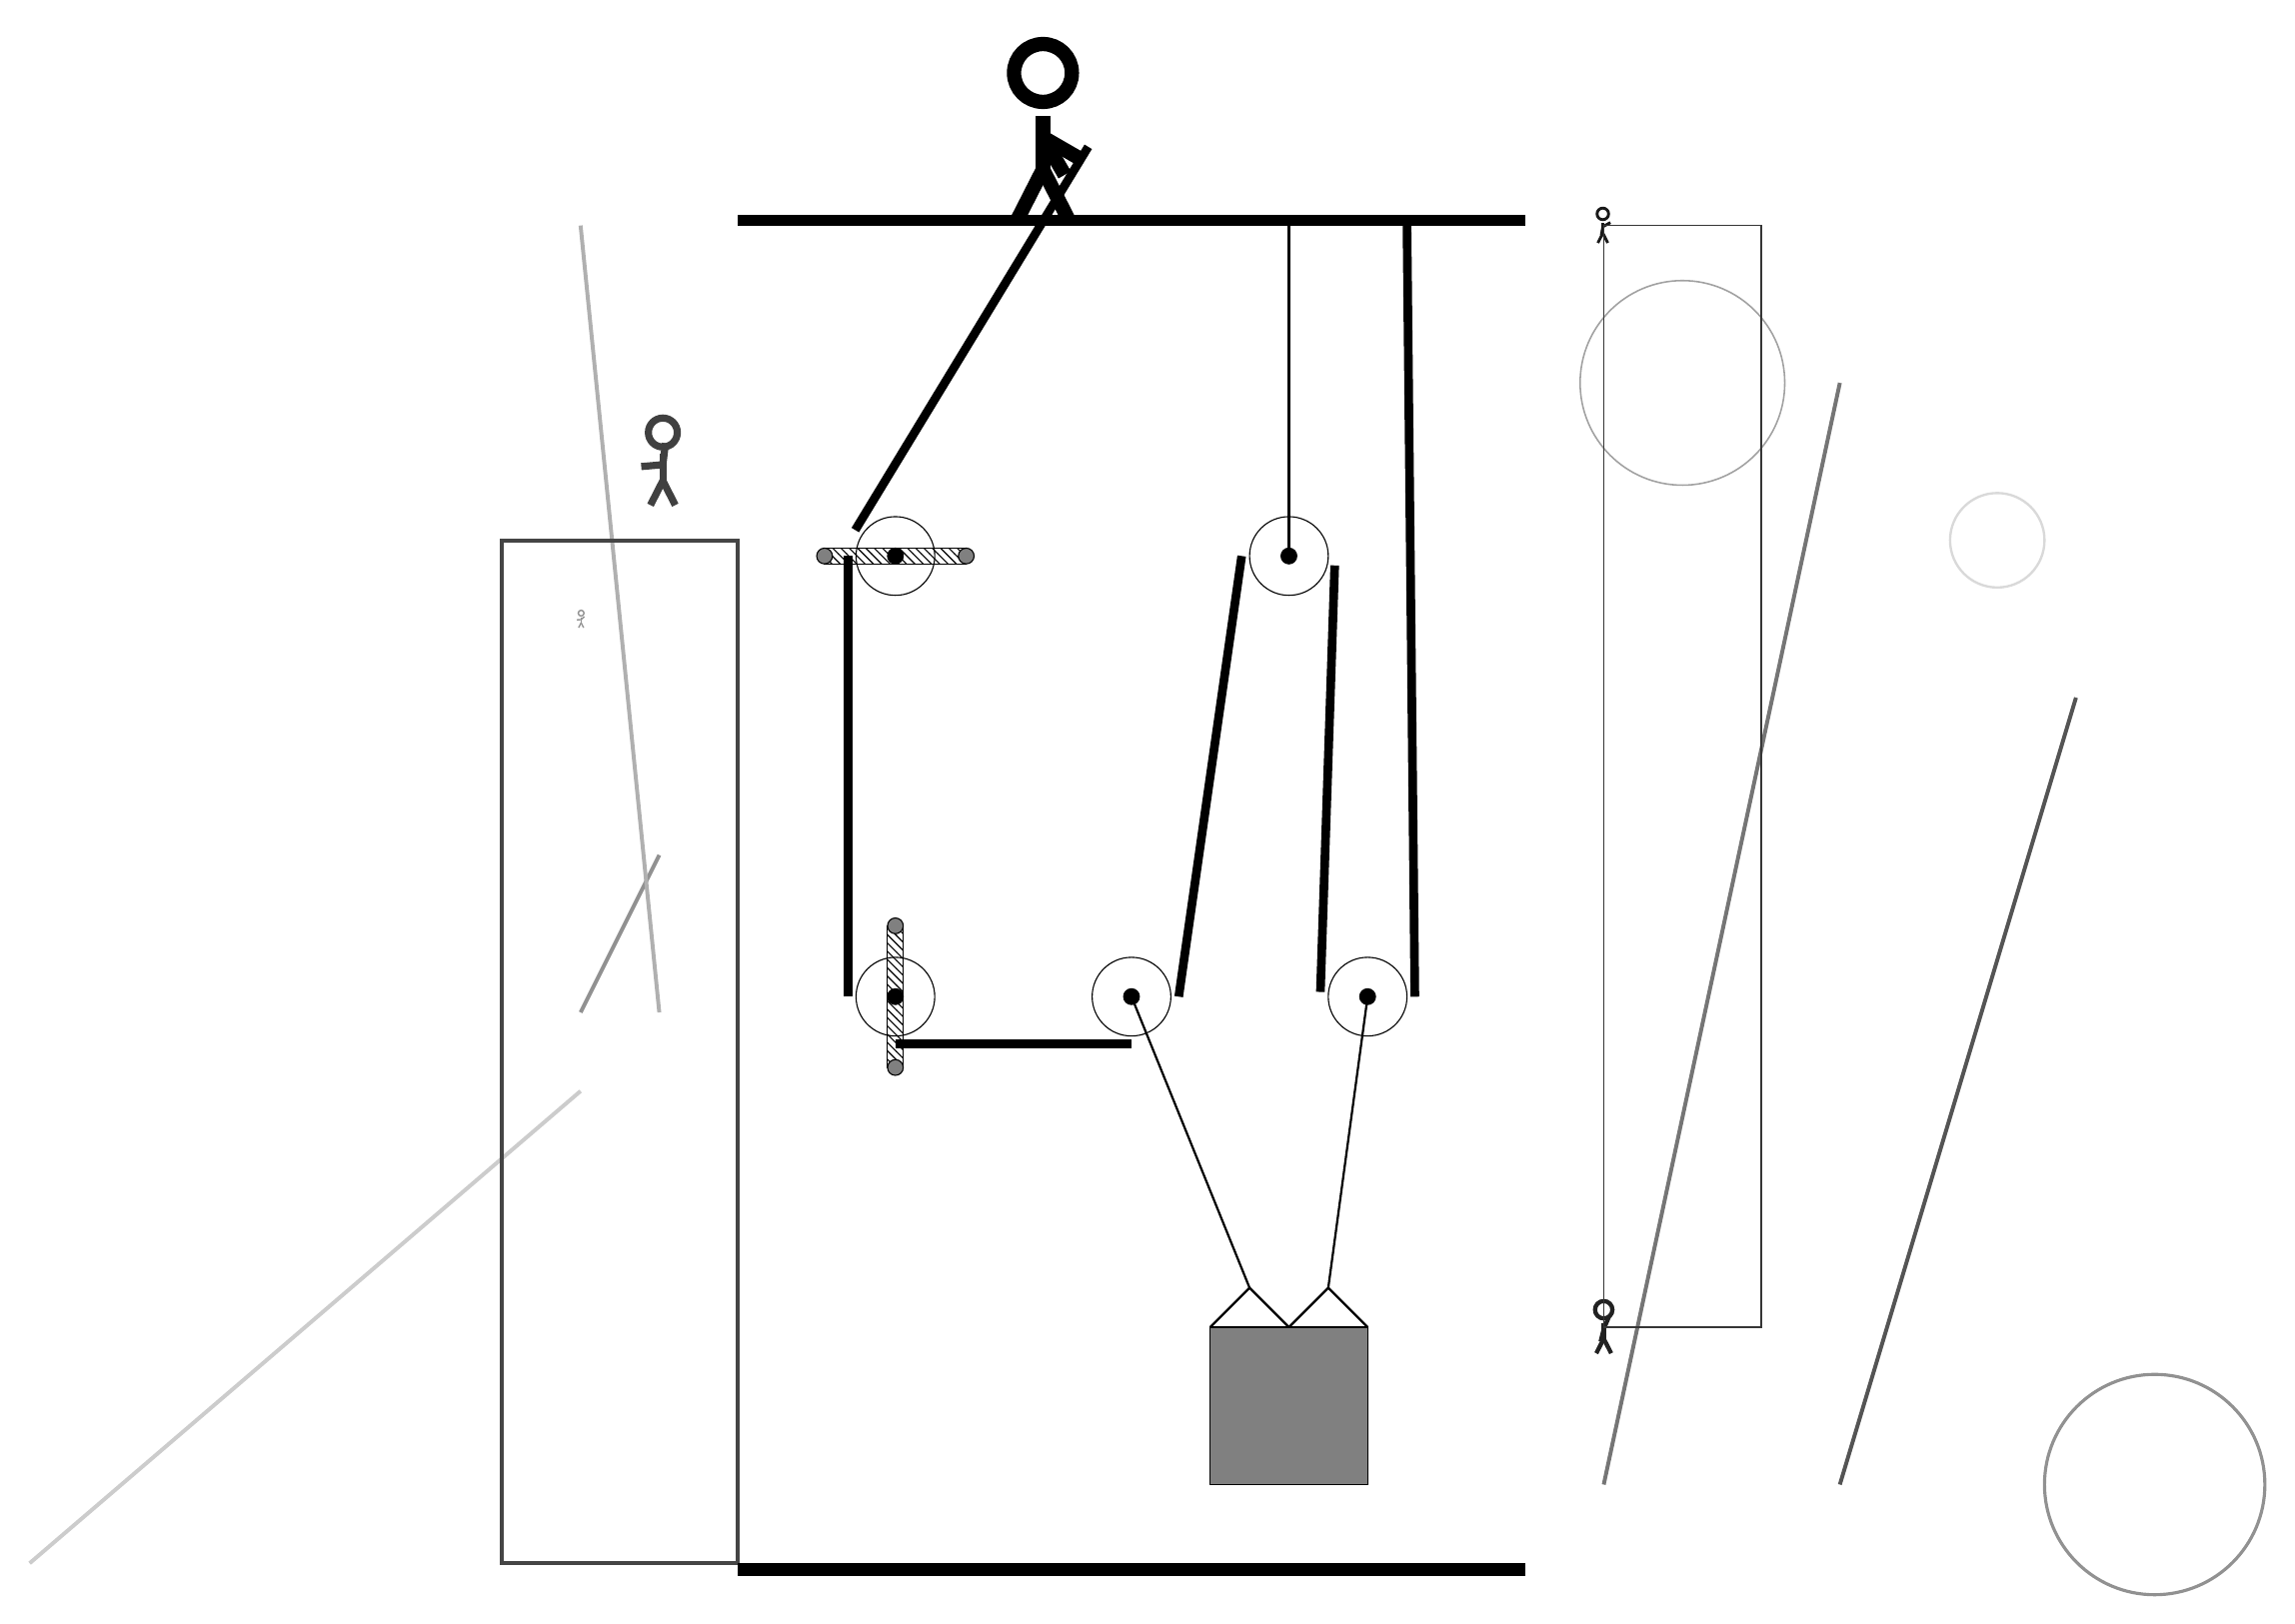
\begin{tikzpicture}
			%%%%% START %%%%%
			
			\draw[fill=black] (-4, 14) rectangle (6, 14.125);
			
			\draw (1, 4.2) circle (0.5);
			\draw[fill=black] (1, 4.2) circle (0.1);
			
			\draw (3, 9.8) circle (0.5);
			\draw[fill=black] (3, 9.8) circle (0.1);
			\draw[thick] (3, 9.8) -- (3, 14);
			
			\draw (4, 4.2) circle (0.5);
			\draw[fill=black] (4, 4.2) circle (0.1);
			
			\draw[thick] (4, 4.2) -- (3.5, 0.5);
			\draw[thick] (1, 4.2) -- (2.5, 0.5);
			\draw[thick]  (2, 0) -- (2.5, 0.5) -- (3, 0);
			\draw[thick]  (3, 0) -- (3.5, 0.5) -- (4, 0);
			\draw[fill=black!50] (2, 0) rectangle (4, -2);
			
			\draw (-2, 4.2) circle (0.5);
			\draw[fill=black] (-2, 4.2) circle (0.1);
			\draw[pattern=north west lines, pattern color=black] (-2.1, 5.1) rectangle (-1.9, 3.3);
			\draw[fill=black!50] (-2, 5.1) circle (0.1);
			\draw[fill=black!50] (-2, 3.3) circle (0.1);
			
			\draw [line width=0.3mm, color=black!76](-6, 5) circle (0.0);
			
			\node[line width=0.7mm, color=black!90] at (7, 14) {\Strichmaxerl[2][80][29]};
			\draw[line width=0.5mm, color=black!43](-5, 6) -- (-6, 4);
			\node[line width=0.4mm, color=black!87] at (7, 0) {\Strichmaxerl[3][76][67]};
			
			\draw[line width=0.5mm, color=black!54](7, -2) -- (10, 12);
			\draw [line width=0.3mm, color=black!15](12, 10) circle (0.6);
			\node[line width=0.2mm, color=black!75] at (-5, 11) {\Strichmaxerl[5][5][83]};
			
			\draw[line width=0.5mm, color=black!20](-6, 3) -- (-13, -3);
			\node[line width=0.6mm, color=black!42] at (-6, 9) {\Strichmaxerl[1][4][42]};
			\draw[line width=0.5mm, color=black!31](-5, 4) -- (-6, 14);
			\draw[line width=0.5mm, color=black!73] (-4, -3) rectangle (-7, 10);
			\draw[line width=0.5mm, color=black!67](10, -2) -- (13, 8);
			\draw [line width=0.2mm, color=black!37](8, 12) circle (1.3);
			
			\draw[line width=0.4mm, color=black!52] (-5, -2) rectangle (-5, -2);
			\draw [line width=0.4mm, color=black!43](14, -2) circle (1.4);
			\draw[line width=0.2mm, color=black!79] (7, 14) rectangle (9, 0);
			
			\draw (-2, 9.8) circle (0.5);
			\draw[fill=black] (-2, 9.8) circle (0.1);
			\draw[pattern=north west lines, pattern color=black] (-2.9, 9.9) rectangle (-1.1, 9.7);
			\draw[fill=black!50] (-2.9, 9.8) circle (0.1);
			\draw[fill=black!50] (-1.1, 9.8) circle (0.1);
			
			\draw[line width=1.1mm] (0.45, 15) -- (-2.51, 10.13);
			\centerarc[line width=1.1mm](-2, 9.8)(135:180:0.6);
			\draw[line width=1.1mm] (-2.6, 9.8) -- (-2.6, 4.2);
			\centerarc[line width=1.1mm](-2, 4.2)(180:270:0.6);
			\draw[line width=1.1mm](-2, 3.6) -- (1, 3.6);
			\centerarc[line width=1.1mm](1, 4.2)(270:360:0.6);
			\draw[line width=1.1mm] (1.6, 4.2) -- (2.4, 9.8);
			\centerarc[line width=1.1mm](3, 9.8)(-20:180:0.6);
			\draw[line width=1.1mm](3.582, 9.68) -- (3.4, 4.26);
			\centerarc[line width=1.1mm](4, 4.2)(160:360:0.6);
			\draw[line width=1.1mm](4.6, 4.2) -- (4.5, 14);
			
			\node at (-0.07, 15.2) {\Strichmaxerl[10][120][-30]};
			
			\draw[fill=black] (-4, -3) rectangle (6, -3.15);
			
			%%%%% END %%%%%
		\end{tikzpicture}
	\end{figure}	
\end{document}